\begin{frame}
\frametitle{Utilidades}
\framesubtitle{Representação eficiente de formas}

Se utilizada uma boa base para representação, é necessária apenas uma parcela da função de base para representar toda a geometria.

\begin{center}
	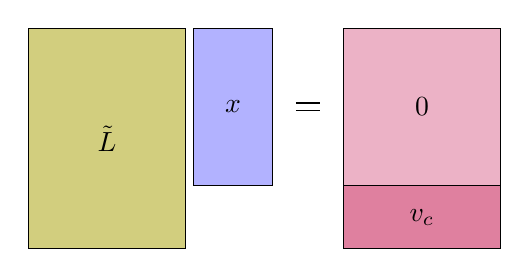
\begin{tikzpicture}
	\filldraw[fill=olive!40!white, draw=black] (0,-0.8) rectangle node{$\tilde{L}$} (2,2);
	\filldraw[fill=blue!30!white, draw=black] (2.1,0) rectangle node{$x$} (3.1,2);
	\draw (3.4, 0.95) -- (3.7, 0.95);
	\draw (3.4, 1.05) -- (3.7, 1.05);
	\filldraw[fill=purple!30!white, draw=black] (4,0) rectangle node{$0$} (6,2);
	\filldraw[fill=purple!50!white, draw=black] (4,0) rectangle node{$v_c$} (6,-0.8);
	\end{tikzpicture}
\end{center}

\end{frame}

\begin{frame}
	\frametitle{Utilidades}
	\framesubtitle{Representação eficiente de formas}
	\begin{figure}
		\centering
		\begin{subfigure}[b]{0.49\textwidth}
			\centering
			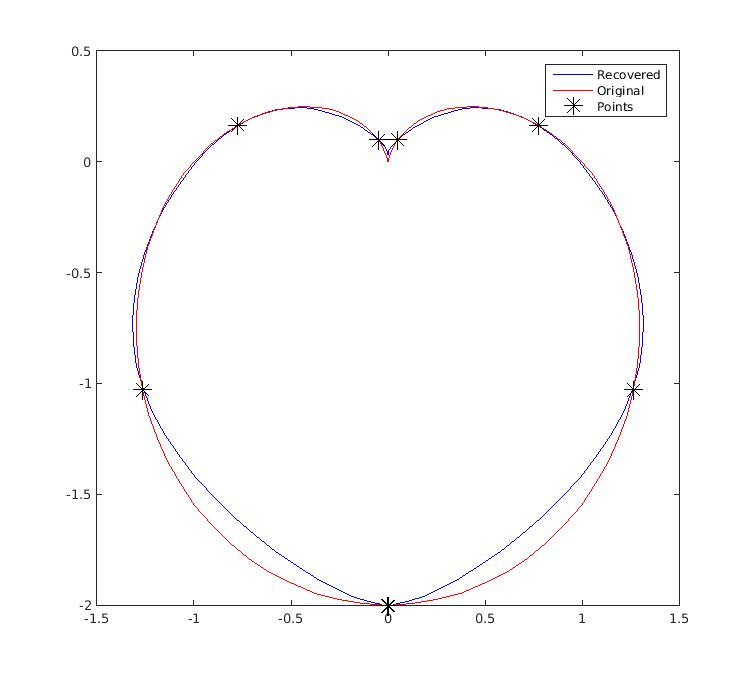
\includegraphics[width=0.9\textwidth]{img/cardioide8.jpg}
			\caption{8 pontos}
			\label{fig:car8}
		\end{subfigure}
		\hfill
		\begin{subfigure}[b]{0.49\textwidth}
			\centering
			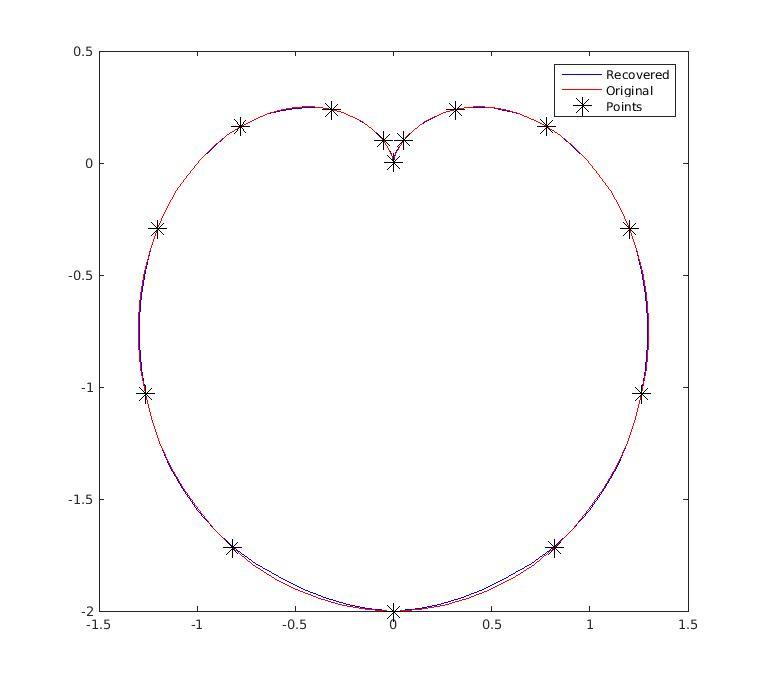
\includegraphics[width=0.9\textwidth]{img/cardioide15.jpg}
			\caption{15 pontos}
			\label{fig:car15}
		\end{subfigure}
		\caption{Reconstrução de cardioides utilizando pontos igualmente espaçados.}
	\end{figure}
\end{frame}

\begin{frame}
	\frametitle{Utilidades}
	\framesubtitle{Representação eficiente de formas}
	\begin{figure}
		\centering
		\begin{subfigure}[b]{0.49\textwidth}
			\centering
			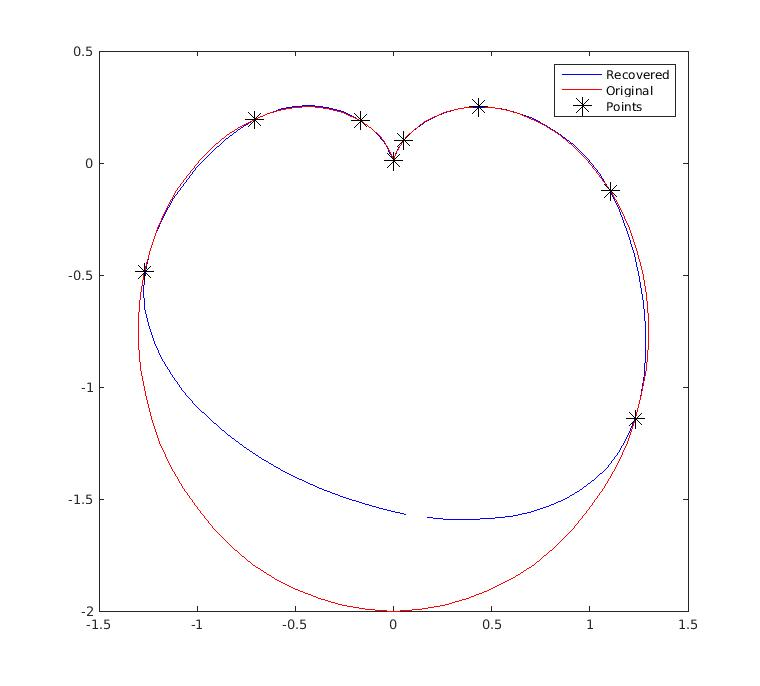
\includegraphics[width=0.9\textwidth]{img/card_curv8.jpg}
			\caption{8 pontos}
			\label{fig:carc8}
		\end{subfigure}
		\hfill
		\begin{subfigure}[b]{0.49\textwidth}
			\centering
			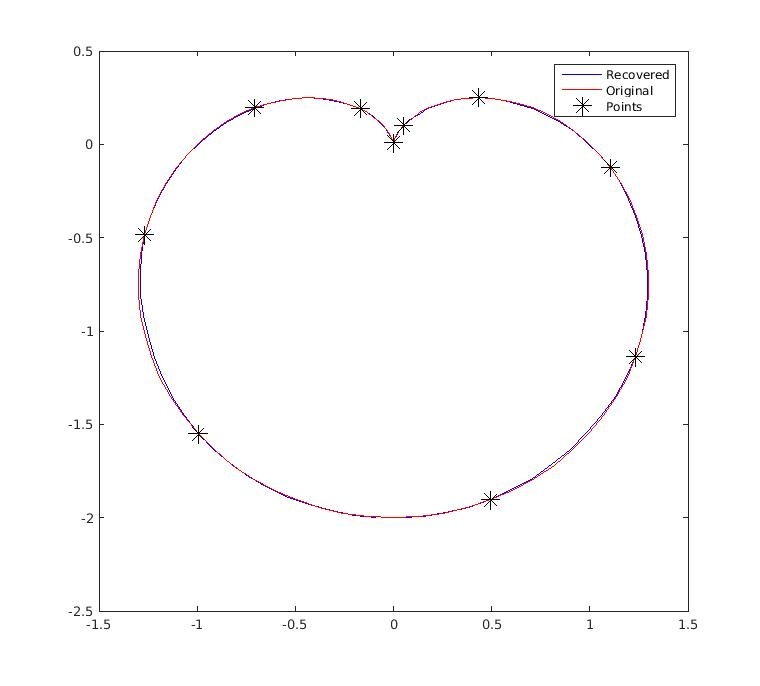
\includegraphics[width=0.9\textwidth]{img/card_curv10.jpg}
			\caption{10 pontos}
			\label{fig:carc10}
		\end{subfigure}
		\caption{Reconstrução de cardioides utilizando pontos com maior curvatura.}
	\end{figure}
\end{frame}

\begin{frame}
\frametitle{Utilidades}
\framesubtitle{Edição de malha e interpolação}

\begin{center}
\begin{figure}
\centering
\begin{subfigure}[b]{0.49\textwidth}
	\centering
	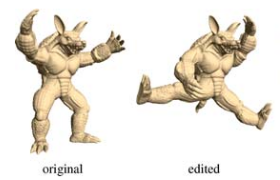
\includegraphics[width=\textwidth]{img/edicao.png}
	\caption{Edição de malhas}
	\label{fig:edic}
\end{subfigure}
\hfill
\begin{subfigure}[b]{0.49\textwidth}
	\centering
	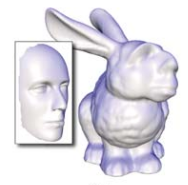
\includegraphics[width=0.7\textwidth]{img/interpolacao.png}
	\caption{Interpolação de malhas}
	\label{fig:interp}
\end{subfigure}

\caption{Exemplos de edição e interpolação \cite{sorkine2006}}
\end{figure}
\end{center}

\end{frame}

%\begin{frame}
%	\frametitle{Códigos}
%	\framesubtitle{Coordenadas diferenciais}
%	
%	\begin{itemize}
%		\item \textbf{genDeltaCoords.m}, geração das $\delta$-coordenadas;
%		\item \textbf{genLaplacian.m}, geração da matriz Laplaciana;
%		\item \textbf{recoverCoords.m}, recuperação das coordenadas cartesianas;
%		\item \textbf{testDelta.m}, testa as funções acima.
%	\end{itemize}
%	
%\end{frame}